\documentclass[tikz]{standalone}
\usepackage{tikz}

\definecolor{codeblack}{RGB}{40, 40, 40}

\definecolor{pinkpic}{RGB}{246, 183, 194}

\tikzstyle{timeline_event}=[align=center, fill=white, inner sep=2pt]

\tikzstyle{timeline_timespan} = [rectangle, draw=codeblack, fill=pinkpic,  text=black,
    text centered, rounded corners, line width=0.4mm]



\begin{document}

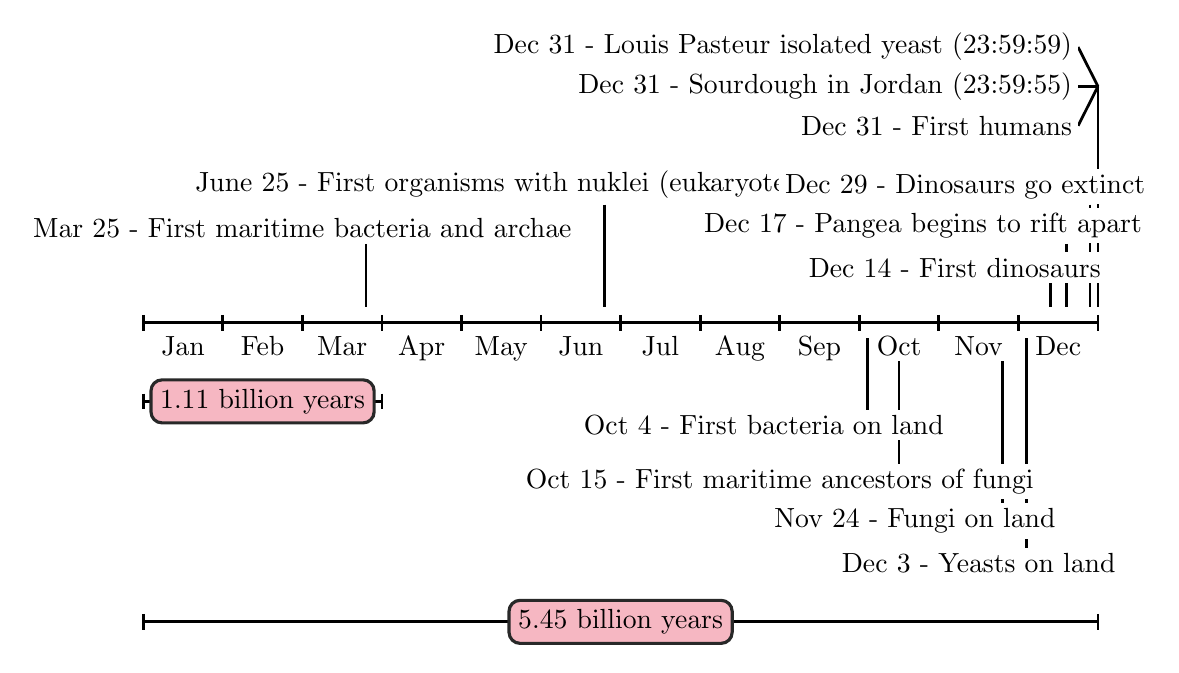
\begin{tikzpicture}
  % Draw horizontal line
  \draw[line width=1pt] (0,0) -- (\textwidth,0);

  % Define the width of each segment
  \pgfmathsetlengthmacro{\segmentwidth}{\textwidth/12}

  % Draw lines for the events, higher up so that they don't overflow the text
  % Placing the lines has been a bit manual work of trying different values
  % Maritime bacteria.

  \draw[line width=1pt] (2.8*\segmentwidth,1) -- (2.8*\segmentwidth,0.2);
  % Eukaryotes
  \draw[line width=1pt] (5.8*\segmentwidth,1.5) -- (5.8*\segmentwidth,0.2);
  % First bacteria on land
  \draw[line width=1pt] (9.1*\segmentwidth,-1.25) -- (9.1*\segmentwidth,-0.2);
  % Maritime fungi ancestors
  \draw[line width=1pt] (9.5*\segmentwidth,-2) -- (9.5*\segmentwidth,-0.2);
  % Fungi on land
  \draw[line width=1pt] (10.8*\segmentwidth,-2.75) -- (10.8*\segmentwidth,-0.2);
  % Yeasts on land
  \draw[line width=1pt] (11.1*\segmentwidth,-3.0) -- (11.1*\segmentwidth,-0.2);
  % First dinosaurs
  \draw[line width=1pt] (11.4*\segmentwidth,0.5) -- (11.4*\segmentwidth,0.2);
  % Pangea begins to rift apart
  \draw[line width=1pt] (11.6*\segmentwidth,1) -- (11.6*\segmentwidth,0.2);
  % Dinosaur extinction
  \draw[line width=1pt] (11.9*\segmentwidth,1.5) -- (11.9*\segmentwidth,0.2);

  % Special lines for december events since they are so close togehter
  \draw[line width=1pt] (12.0*\segmentwidth,3.0) -- (12.0*\segmentwidth,0.2);  % Main branch
  \draw[line width=1pt] (12.0*\segmentwidth,3.0) -- (11.75*\segmentwidth,2.5); % Branch to first humans
  \draw[line width=1pt] (12.0*\segmentwidth,3.0) -- (11.75*\segmentwidth,3.0); % Branch to Jordan
  \draw[line width=1pt] (12.0*\segmentwidth,3.0) -- (11.75*\segmentwidth,3.5); % Branch to Pasteur

  % Draw months and month separators
  \foreach \i/\month in {0/Jan, 1/Feb, 2/Mar, 3/Apr, 4/May, 5/Jun, 6/Jul, 7/Aug, 8/Sep, 9/Oct, 10/Nov, 11/Dec} {
      % Separators
      \draw[line width=1pt] (\i*\segmentwidth,0.1) -- (\i*\segmentwidth,-0.1);
      % Month names
      \node[timeline_event, below] at ({(\i+0.5)*\segmentwidth},-0.1) {\month};
  }
  \draw[line width=1pt] (\textwidth,0.1) -- (\textwidth,-0.1);

  % Full timeline width for billion years
  \draw[line width=1pt] (0,-3.8) -- node[midway, timeline_timespan] {5.45 billion years} (\textwidth,-3.8);
  \draw[line width=1pt] (0,-3.7) -- (0,-3.9);
  \draw[line width=1pt] (\textwidth,-3.7) -- (\textwidth,-3.9);

  % Indicator for the period of 3 months = 1.1 billion years
  \draw[line width=1pt] (0,-1.0) -- node[midway, timeline_timespan] {1.11 billion years} ({\segmentwidth * 3},-1.0);
  \draw[line width=1pt] (0,-0.9) -- (0,-1.1);
  \draw[line width=1pt] ({\segmentwidth * 3},-0.9) -- ({\segmentwidth * 3},-1.1);

  % Place events on the timeline with dates using the timeline_event style
  % As a calculation I used (4.54 billion years / 12 months = 0.3785 billion years/month.
  \node[timeline_event, above] at (2.0*\segmentwidth,1) {Mar 25 - First maritime bacteria and archae};
  \node[timeline_event, above] at (4.50*\segmentwidth,1.5) {June 25 - First organisms with nuklei (eukaryotes)};
  \node[timeline_event, above] at (7.8*\segmentwidth,-1.5) {Oct 4 - First bacteria on land};
  \node[timeline_event, above] at (8.0*\segmentwidth,-2.25) {Oct 15 - First maritime ancestors of fungi};
  \node[timeline_event, above] at (9.7*\segmentwidth,-2.75) {Nov 24 - Fungi on land};
  \node[timeline_event, above] at (10.5*\segmentwidth,-3.25) {Dec 3 - Yeasts on land};
  \node[timeline_event, above] at (10.2*\segmentwidth,0.5) {Dec 14 - First dinosaurs};
  \node[timeline_event, above] at (9.8*\segmentwidth,1) {Dec 17 - Pangea begins to rift apart};
  \node[timeline_event, above] at (10.33*\segmentwidth,1.5) {Dec 29 - Dinosaurs go extinct};
  \node[timeline_event, above, anchor=east, align=right] at (11.75*\segmentwidth,2.5) {Dec 31 - First humans};
  \node[timeline_event, above, anchor=east, align=right] at (11.75*\segmentwidth,3.0) {Dec 31 - Sourdough in Jordan (23:59:55)};
  \node[timeline_event, above, anchor=east, align=right] at (11.75*\segmentwidth,3.5) {Dec 31 - Louis Pasteur isolated yeast (23:59:59)};

\end{tikzpicture}
\end{document}
